%!TEX root = ../main.tex
\section{Descriptive Data Analytics of COVID-19}
\label{sec:descriptive}

%\stitle{Linked Visualizations.}



Visualization selection generates three categories of charts: {\em linked} common visualizations, {\em ad-hoc} visualizations, and {\em recommended} visualizations.

\stitle{(General) Linked Visualizations.} There are common visualizations for spatio-temporal data exploration, such as a choropleth map (a heat map based on a map), line charts to show various trends, bar charts to show the comparison between various groups, scatter charts (or bubble charts) to quantify the relationship between two quantitative variables (\eg death rate vs. cure rate).
We carefully selected charts (see Figure~\ref{fig:frontend}) that can attract a wide range of interest, and make them ``linked'', \eg when one zoom in from a world level to a country level, all the other charts will be zoomed in, so as to provide a synchronized view from multiple charts.
%%%%
%%%%
The user can get high-level situations of COVID-19 from Figure~\ref{fig:frontend}.
For example, the user can catch the overall information of the reported cases from Figure~\ref{fig:frontend}(A).
%
The choropleth map in Figure~\ref{fig:frontend}(B) shows the location and number of confirmed cases, deaths and recoveries for all affected countries. It also provides a timeline toolbar for the user to look back upon previous situations, and a user can click the ``$\blacktriangleright$'' button to show an animation.
%
The user can click a country, \eg China, to drill down into the country-level (province-level or city-level) for more details. Since we apply the linked visualization techniques, the rest of the visualizations will also drill down into the country-level.
%
Figure~\ref{fig:frontend}(C), a line chart, illustrates the daily increased cases of the selected location.
%
The stacked bar chart in Figure~\ref{fig:frontend}(D) depicts the number of cases for the selected location.
%
The pie charts in Figure~\ref{fig:frontend}(E) show the proportion of patients' type.
% 
Figure~\ref{fig:frontend}(F), a bubble chart, illustrates the relationships across \#-cases, deaths rate, and cure rate.
%
The bar chart in Figure~\ref{fig:frontend}(G) shows the distribution of patients' age, and the calendar chart in Figure~\ref{fig:frontend}(H) illustrates the proportion of types of reported cases for each day.


%\add{You can copy the description of the demo paper bout A--H to give more details.}



%%%%%%%%%%%%%%%%%%%%%%%%%%%%%%%%%%%%
\begin{figure}[t!]
	\centering
	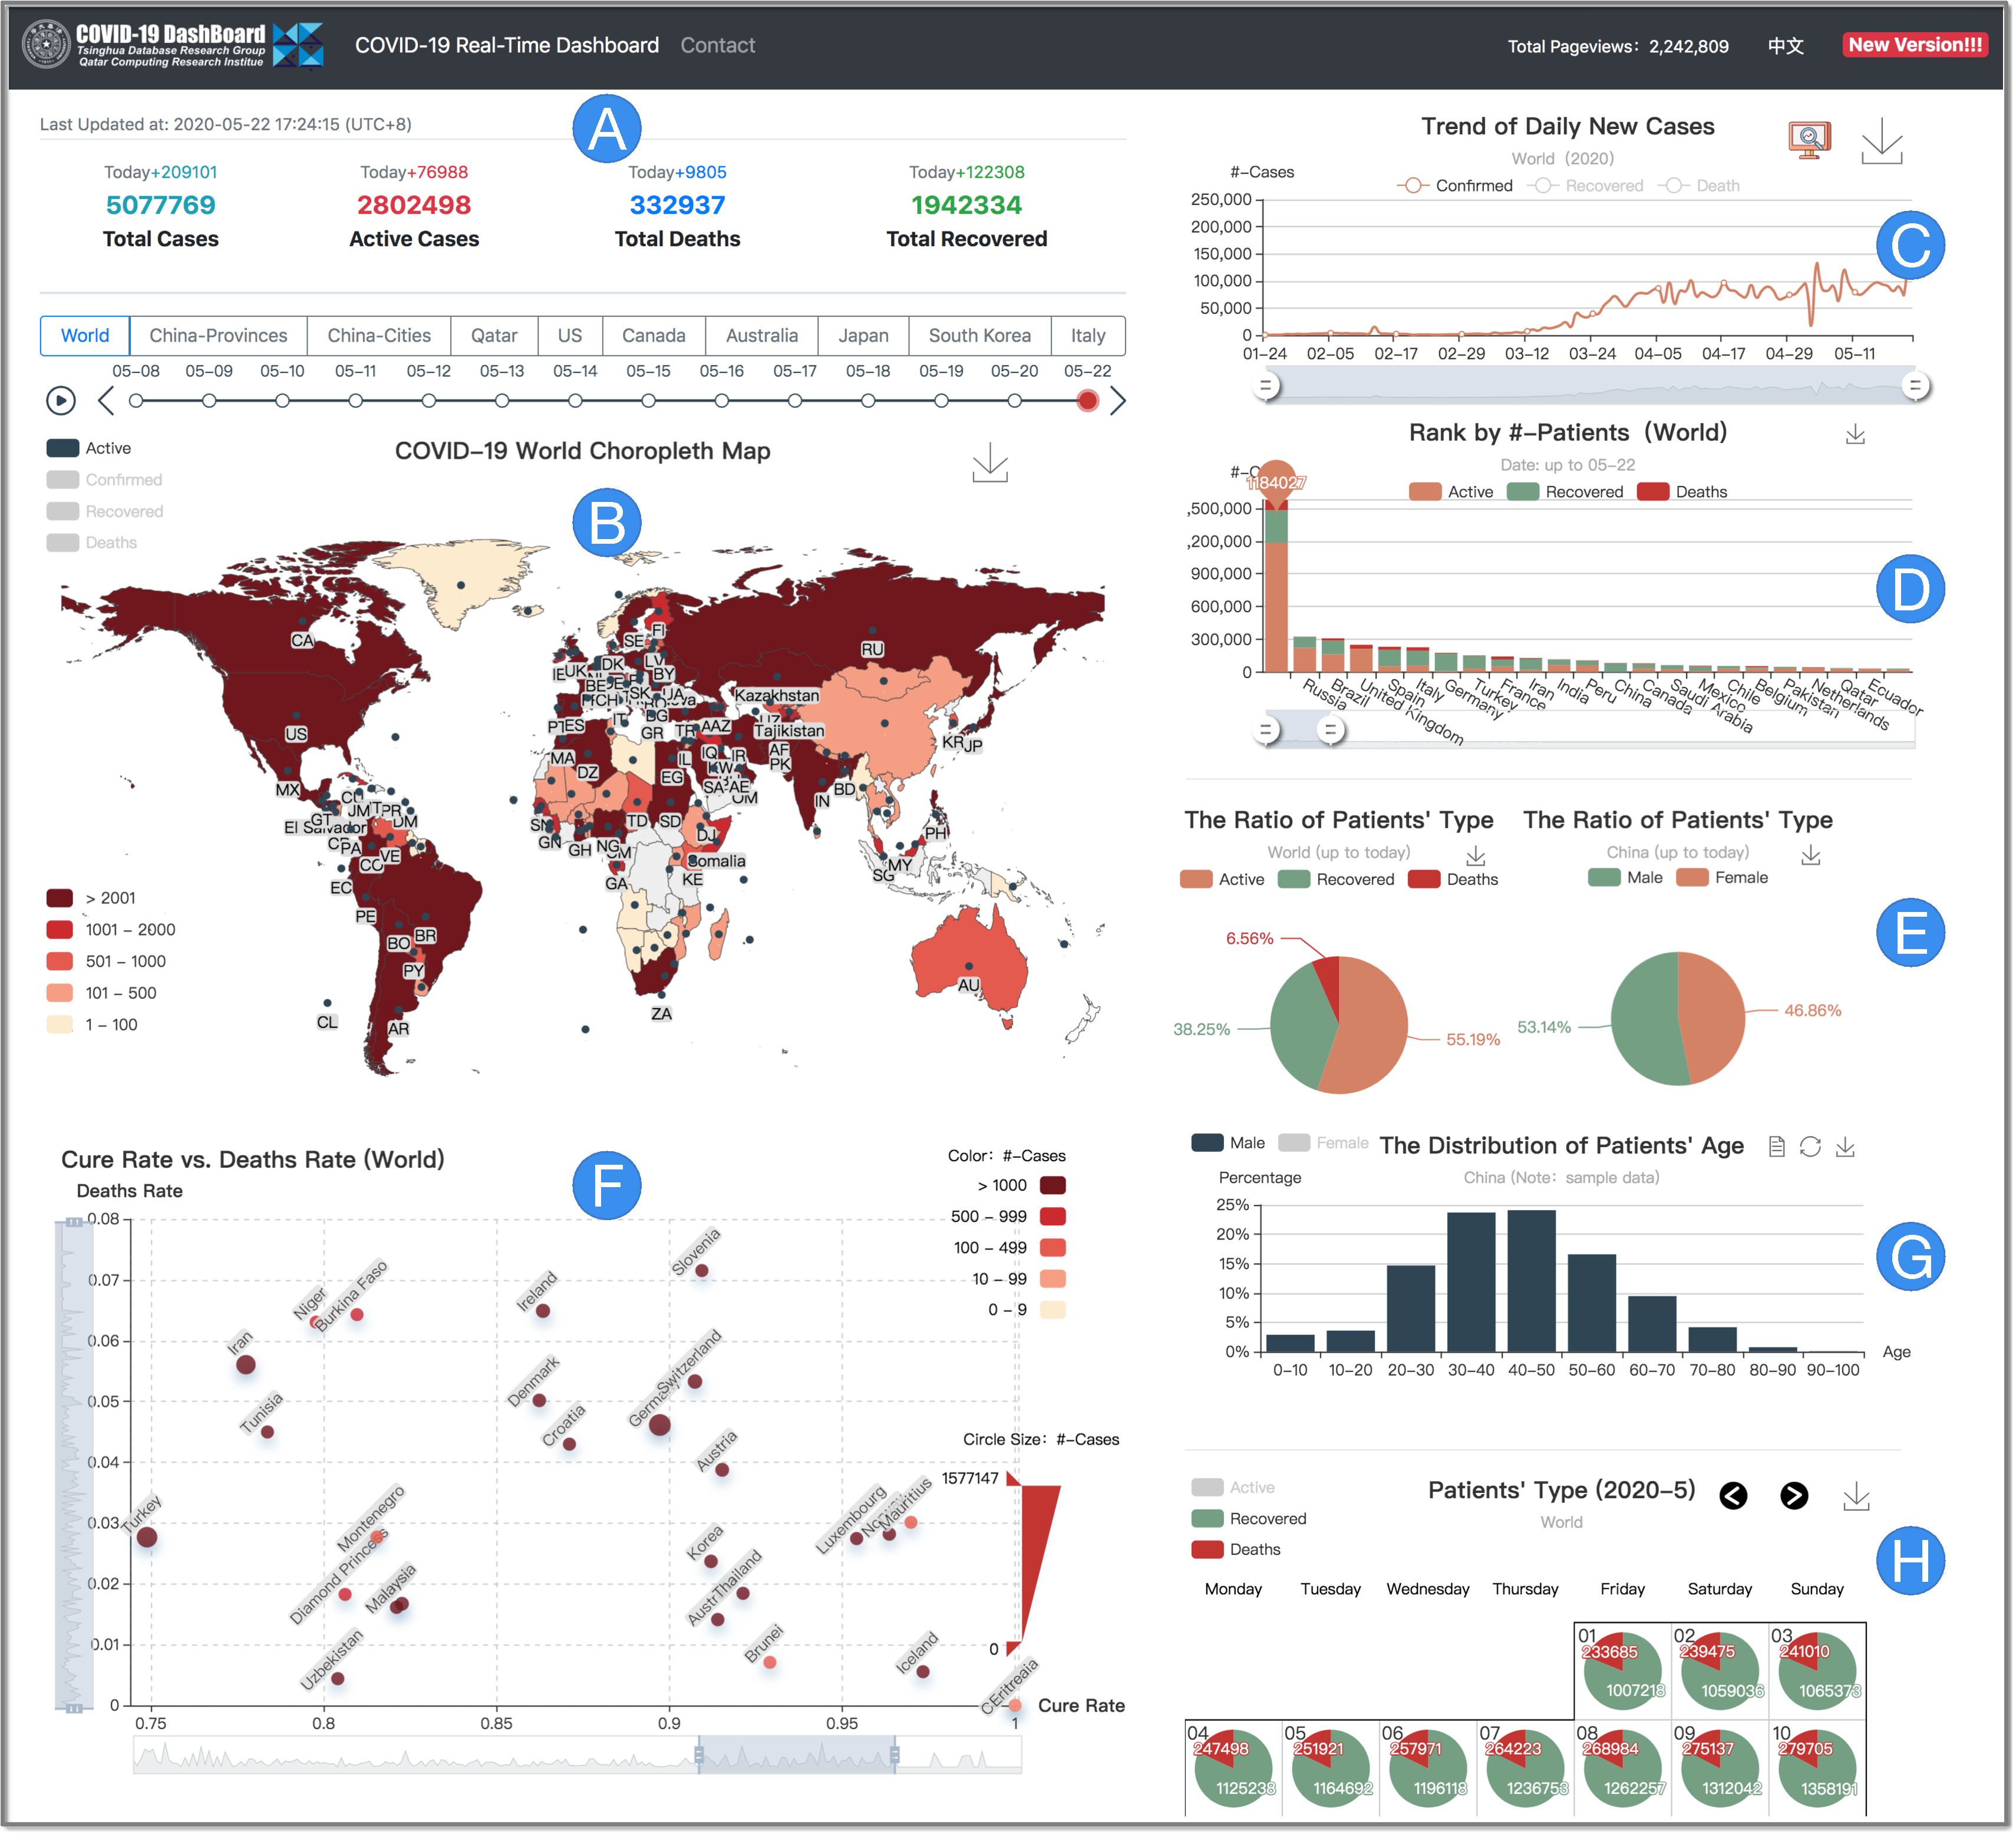
\includegraphics[width=.95\columnwidth]{figs/frontend.pdf}
	\vspace{-1em}
	\caption{The Frontend of \sys (\lgl{https://ncov.deepeye.tech/en})}
	\label{fig:frontend}
	\vspace{-1em}
\end{figure}
%%%%%%%%%%%%%%%%%%%%%%%%%%%%%%%%%%%


%%%%%%%%%%%%%%%%%%%%%%%%%%%%%%%%%%%%
\begin{figure*}[t!]
	\begin{minipage}{\textwidth}
		\centering
		\begin{minipage}{0.4\textwidth}
			\begin{figure}[h]
				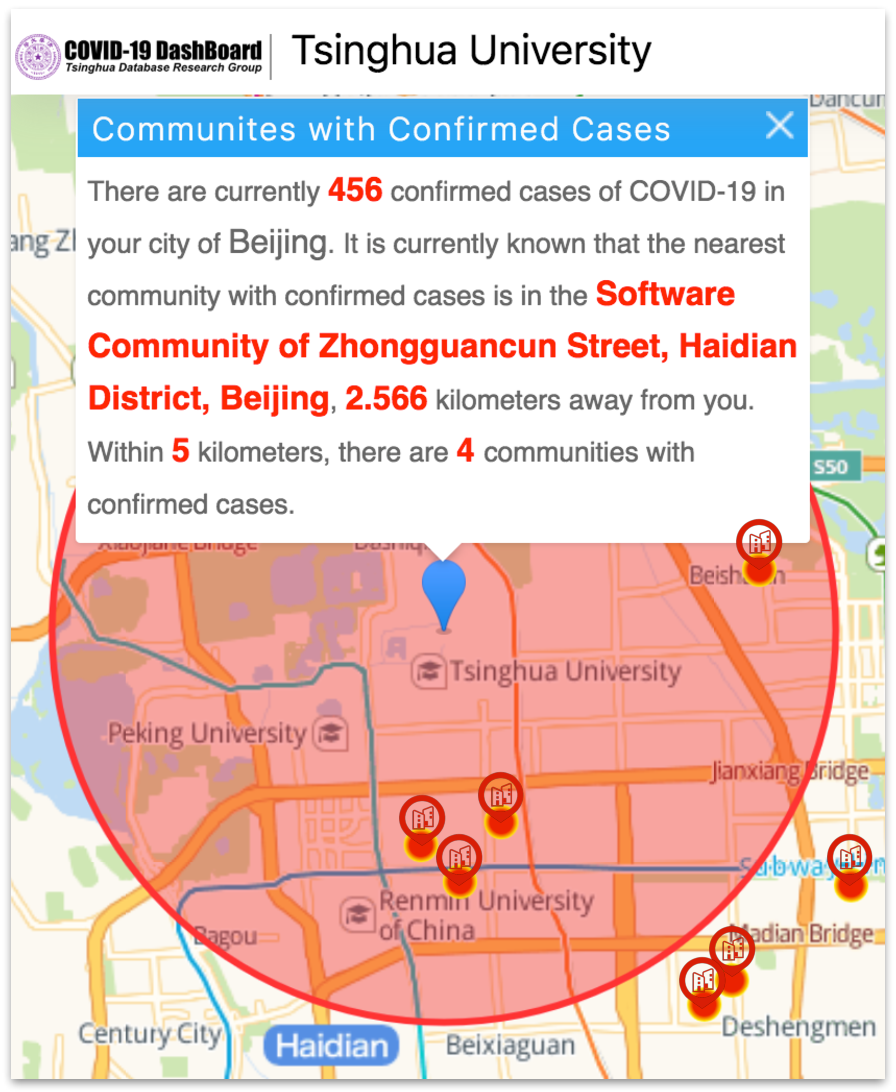
\includegraphics[width=\columnwidth]{{figs/community.pdf}}
				\caption{Find Confirmed Cases Around You}
				\label{fig:community}		
			\end{figure}
		\end{minipage}
		\begin{minipage}{0.59\textwidth}
			\begin{figure}[h]
				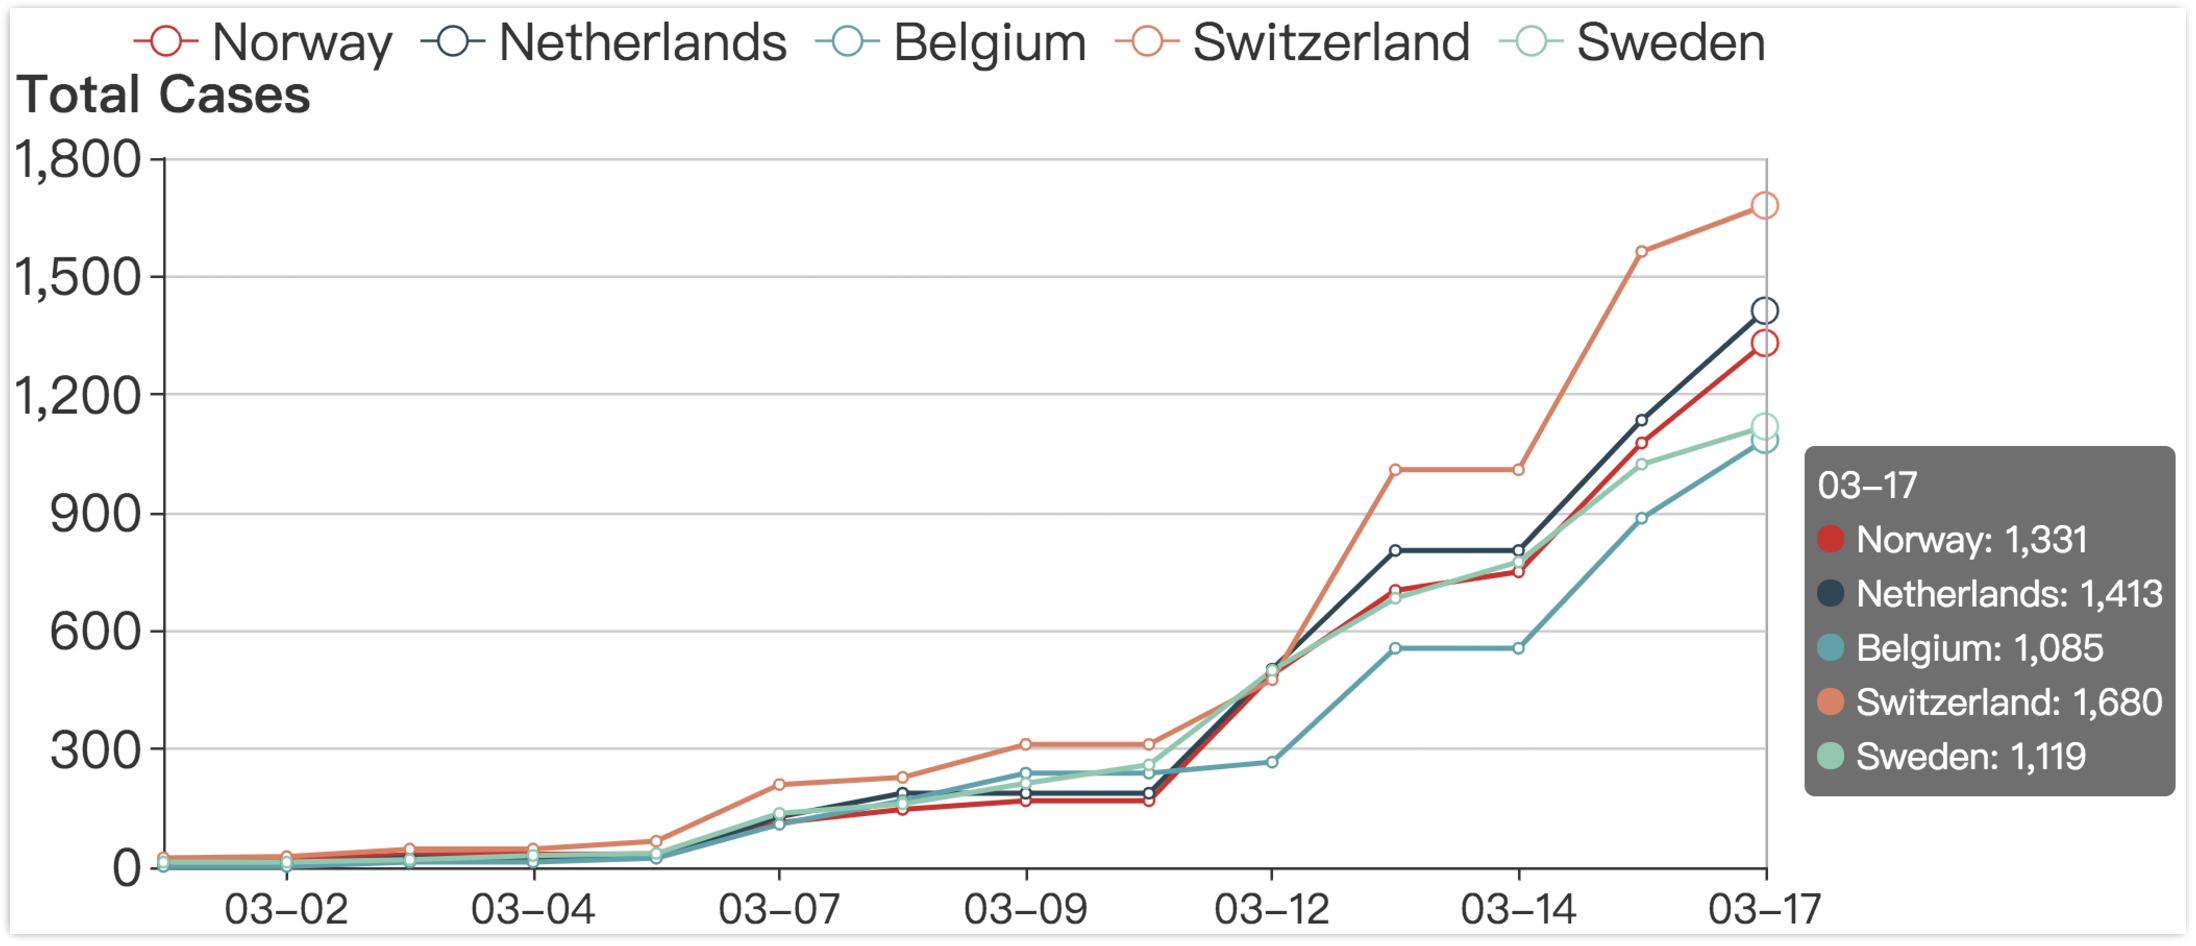
\includegraphics[width=\columnwidth]{figs/similarity_trend1.pdf}
				\caption{Similar Trend of Confirmed Cases}
				\label{fig:similar_trend}
			\end{figure}
		\end{minipage}
	\end{minipage}
\end{figure*}
%%%%%%%%%%%%%%%%%%%%%%%%%%%%%%%%%%%%


%%%%%%%%%%%%%%%%%%%%%%%%%%%%%%%%%%%%
\begin{figure}[t!]
	\centering
	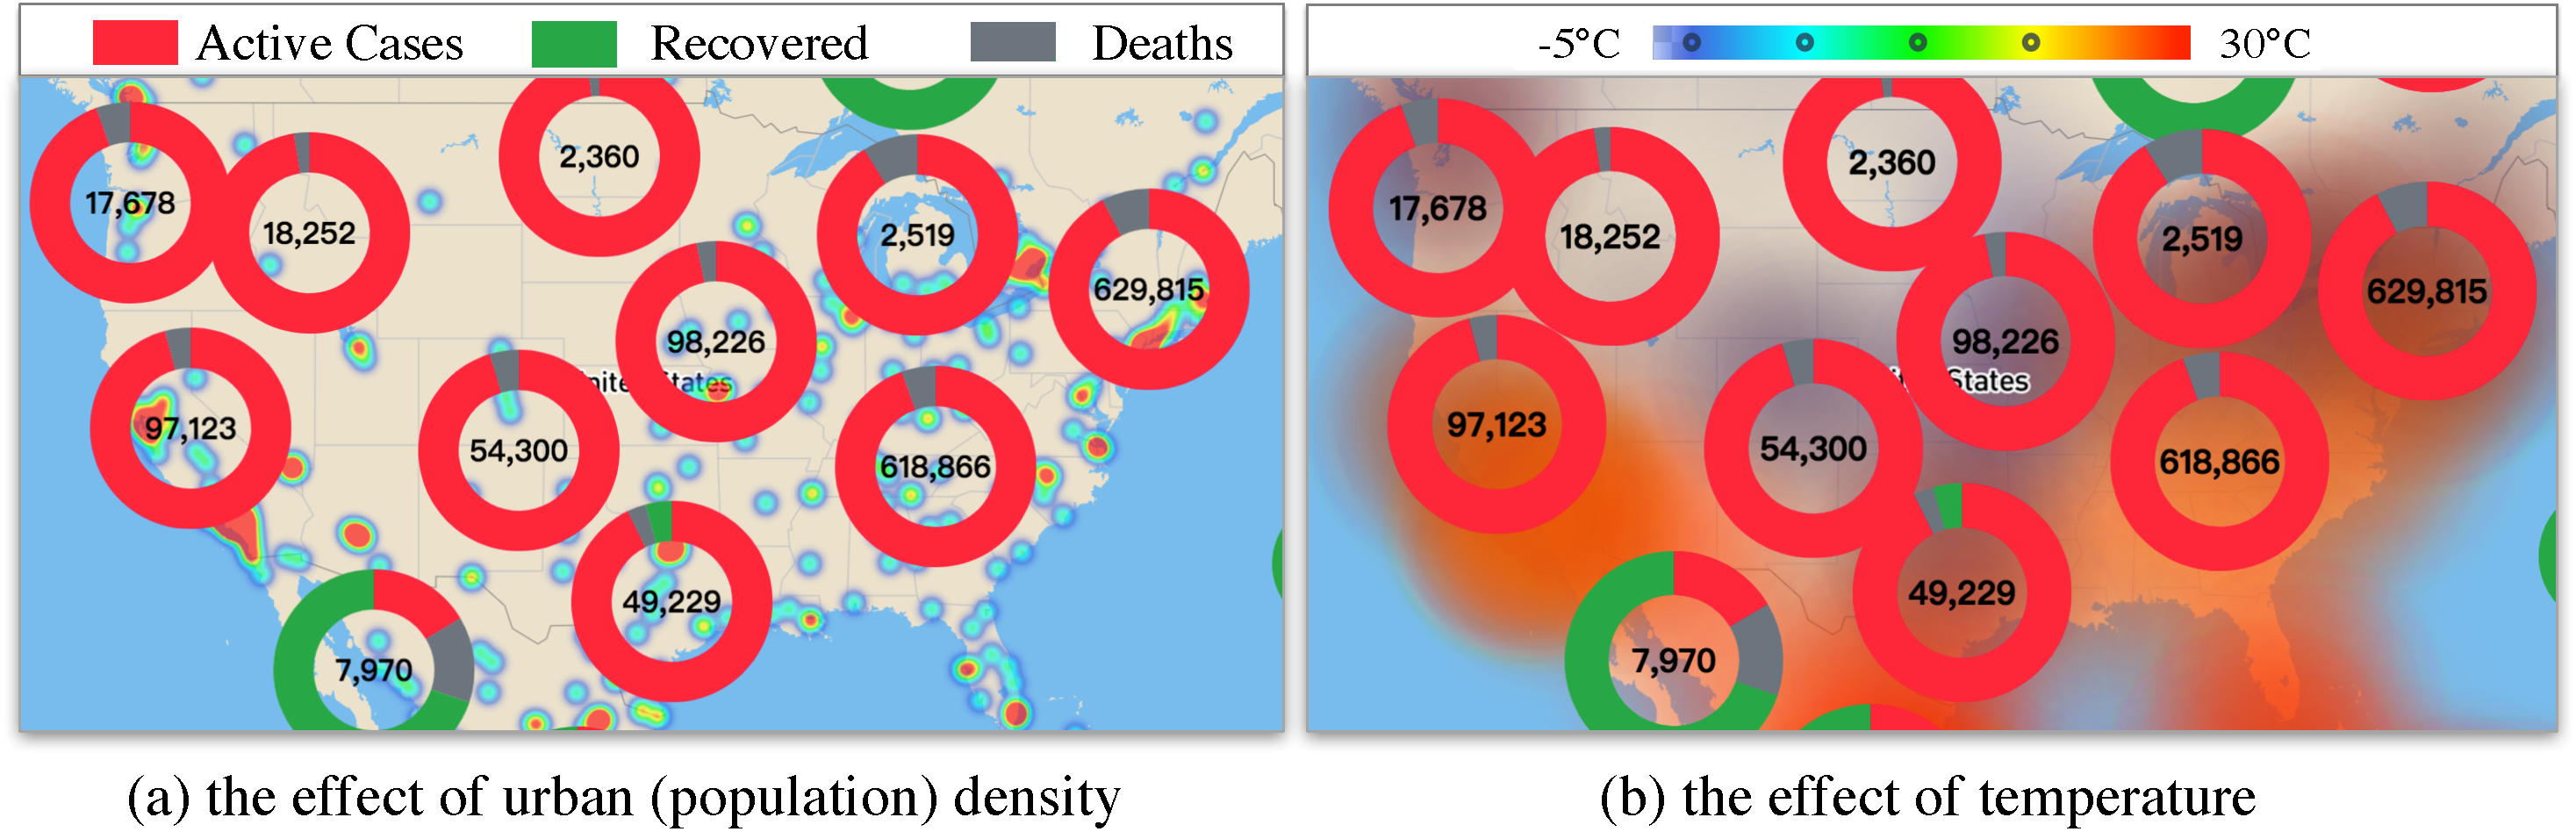
\includegraphics[width=1\columnwidth]{figs/urban_temp.pdf}
	\vspace{-2em}
	\caption{Diagnostic Data Analytics (Case in United States)}
	\label{fig:diagnostic}
	\vspace{-1em}
\end{figure}
%%%%%%%%%%%%%%%%%%%%%%%%%%%%%%%%%%%

\stitle{Location-based Search.}
For the general public, \sys provides the module of finding confirmed cases in nearby neighborhoods. 
Take Figure~\ref{fig:community} for example, users can understand the COVID-19 situations near {\em Tsinghua University, Beijing, China} by a location search box. Note that this module only supports for the Mainland China area currently.

\stitle{Similarity Trends Discovery.}
\sys also supports the similar trend search functionality for finding similar trends. 
%This feature is supported by {\sc DeepEye}~\cite{deepeyeicde} in the back-end.
For example, if the user wants to find those trends of confirmed cases that are similar to {\em Switzerland}, the similarity search functionality will return top-$k$ similar trends about {\em Switzerland}.
The running example is shown in Figure~\ref{fig:similar_trend}. 
Besides line charts,  the similar trend search also supports other charts (\eg bar chart and pie chart).
Thanks to this functionality,  users can perform comparative analysis easier.

\stitle{Automatic News Generation.}
Automatic news generation, in other words, automatically extracting insights from data visualization is promising research and practical direction~\cite{DBLP:journals/vldb/QinLTL20}.
Currently, the user usually interacts with the visualization dashboard to get insights and make decisions. 
For example, the reporter may interact with the dashboard to observe the trend of daily new confirmed cases of each country/state and find a set of similar trends (or find a set of rapidly increasing trends) as news stories.
In this scenario, it heavily relies on the user to manually get insights and write a news release.
One intuitive idea is whether we can derive insights (news stories) from the visualization dashboard automatically. 
%
Roughly speaking, given a set of visualizations $\mathbf{V}$ and a news generation model $\mathbf{M}$, the automatic news generation problem is to output a set of new stories $\mathbf{S}$. 
The key challenge is how to design the news generation model $\mathbf{M}$.
One straightforward approach is predefined a set of expert knowledge rules to mine insights from the visualization dashboard.
%
Such rules can be similar trends discovery, outlier trend detection, trends comparison, and so on.





